
%% bare_conf.tex
%% V1.4b
%% 2015/08/26
%% by Michael Shell
%% See:
%% http://www.michaelshell.org/
%% for current contact information.
%%
%% This is a skeleton file demonstrating the use of IEEEtran.cls
%% (requires IEEEtran.cls version 1.8b or later) with an IEEE
%% conference paper.
%%
%% Support sites:
%% http://www.michaelshell.org/tex/ieeetran/
%% http://www.ctan.org/pkg/ieeetran
%% and
%% http://www.ieee.org/
%%*************************************************************************
%% Legal Notice:
%% This code is offered as-is without any warranty either expressed or
%% implied; without even the implied warranty of MERCHANTABILITY or
%% FITNESS FOR A PARTICULAR PURPOSE!
%% User assumes all risk.
%% In no event shall the IEEE or any contributor to this code be liable for
%% any damages or losses, including, but not limited to, incidental,
%% consequential, or any other damages, resulting from the use or misuse
%% of any information contained here.
%%
%% All comments are the opinions of their respective authors and are not
%% necessarily endorsed by the IEEE.
%%
%% This work is distributed under the LaTeX Project Public License (LPPL)
%% ( http://www.latex-project.org/ ) version 1.3, and may be freely used,
%% distributed and modified. A copy of the LPPL, version 1.3, is included
%% in the base LaTeX documentation of all distributions of LaTeX released
%% 2003/12/01 or later.
%% Retain all contribution notices and credits.
%% ** Modified files should be clearly indicated as such, including  **
%% ** renaming them and changing author support contact information. **
%%*************************************************************************



\documentclass[a4paper,conference]{IEEEtran}

\def\citepunt{,}

\usepackage[pdftex]{graphicx}
\ifCLASSOPTIONcompsoc
  \usepackage[caption=false,font=normalsize,labelfont=sf,textfont=sf]{subfig}
\else
  \usepackage[caption=false,font=footnotesize]{subfig}
\fi
\usepackage{comment}
\usepackage{float}
\usepackage{mathtools}
\usepackage{amsfonts}
\usepackage{bm}

\DeclarePairedDelimiter\ceil{\lceil}{\rceil}
\DeclarePairedDelimiter\floor{\lfloor}{\rfloor}

\newcommand{\R}{\mathbb{R}}
\newcommand{\A}{\mathcal{A}}
\newcommand{\D}{\mathcal{D}}
\newcommand{\I}{\hat{I}}
\newcommand{\Z}{\mathbb{Z}}
\newcommand{\m}[1]{{\mathrm{\bf #1}}}
\newcommand{\E}{\tilde{\m{I}}}
\newcommand{\F}{\hat{F}}
\newcommand{\lI}{\m{I}}
\newcommand{\mF}{\m{F}}
\newcommand{\bF}{\mathcal{F}}
\newcommand{\J}{\hat{J}}
\newcommand{\lJ}{\m{J}}
\newcommand{\pD}{D^\prime}
\newcommand{\eF}{\hat{\mF}}
\newcommand{\gN}{\m{N}}
\newcommand{\W}{\m{W}}
\newcommand{\M}{\mathcal{M}}
\newcommand{\Pa}{\mathcal{P}}
\newcommand{\pDD}{\D^\prime}

% correct bad hyphenation here
\hyphenation{op-tical net-works semi-conduc-tor}


\begin{document}

\title{Learning filters from user provided image makers}

% make the title area
\maketitle

\begin{abstract}
    
\end{abstract}

\section{Introduction}
Deep learning has proven to be applicable to different types of tasks, from image classification to the creation of synthetic data \cite{goodfellow2016deep}. Given the success of the application of deep learning in various areas of knowledge, this technique has also been applied to several tasks of remote sensing. Examples of this technique exist in various problems such as segmentation of terrain images \cite{kemker2018algorithms, kampffmeyer2016semantic, hamaguchi2018effective}, building identification \cite{xu2018building, lu2018detecting, liu2018multilevel}, and deforestation monitoring \cite{bragilevsky2017deep}. 

The detection of trees is important to produce knowledge about the land use of a region, from the assessment of crop diversity or the performance of plantations in a given season to the assessment of damages after natural disasters such as drilling and flooding. As these plantations can span very large areas, manual detection can be costly and susceptible to errors. 

In \cite{fassnacht2016review}, we can see a review of the problem of classification of tree species of aerial images. \cite{puttemans2018comparing} apply deep learning to the problem of detecting coconut trees in aerial images. Aparta et al. \cite{aparna2018cnn} apply convolutional neural networks to count coconut trees on plantations in India. Vargas-Muñoz et al. \cite{8899005} propose an active learning approach to detect coconut trees that seeks to reduce the effort of annotating images. The \cite{8899005} approach is divided into a stage of producing candidate patches for having a coconut tree and a stage where a CNN determines whether a patch has a coconut tree. We propose a different way to produce this classifier.  

Despite this success, methods based on deep learning require a lot of annotated images for training, and annotating this volume of data is quite costly. Even interactive methods require large training sets. If these methods depend on huge training sets, their application may not be feasible in areas where it is impossible, or the cost of gathering and annotating these data sets is prohibitive. Much of the user's interaction with methods based on deep learning occurs through the annotation of the training set, and the user does not have much influence on the training process.

Despite the advances in deep learning over the last decades, especially with most recent deep neural networks, some important questions related to human interaction remain unanswered: (1) How to choose the most reasonable model, in the sense that it provides acceptable effectiveness, being as simple and efficient as needed, for a given classification problem? (2) How to train that model from a reduced number of samples?  (3) Can the user explain the decisions of that model? (4) Can that model improve from human corrections? The first question requires to explore human knowledge about the classification technique and the problem of interest. The second one requires to reduce as much as possible the human effort to train a model. The third issue is related to human understanding, and it may explore techniques (such as data visualization) to explain the decisions of the model and perhaps to guide human decisions concerning the design of the model. The fourth question is also important during training, and it is related to human control over the process. They all lead to the importance of involving human experts during the machine learning process.

In this paper, we present some advances towards the answers to the questions (1) and (2). We also discuss future research related to the questions (3) and (4). We present a method to the design of light-weighted convolutional neural networks from markers drawn by an expert on a few images to indicate representative regions of each object of interest for classification. From those markers, our approach can learn the filters of each layer, and the convolutional neural network can be designed in a layer-by-layer fashion, with no need for backpropagation in order to build a representative feature space for the classification problem. Backpropagation is only used to train a bank of multi-layer perceptrons for local pattern classification.

We propose a new way of learning the filters of the convolutional layers of deep neural networks that do not depend on the optimization of an error function and, therefore, do not need a large number of training samples. The training process is done with user intervention, which adds markers to the training images to indicate relevant features to characterize each class. To learn the filters, we get a patch around each marker of a class and cluster them. The centroid of each cluster is a filter that can be used to identify features of this cluster. The set of centroids of clusters of all clusters is the convolutional layer filters. For the next layer, the patches are generated on the output of the previous one. To evaluate our method, we use a dataset of aerial images to detect coconut trees. We identified that, with few layers and few training samples, we managed to get competitive results with state-of-the-art models.


\section{Learning filters from markers}
Our method is based on the idea that the network designer is an expert in the application domain or knows well enough to indicate which are the relevant characteristics of the objects of interest. The designer highlights these regions by placing markers, which are associate to pixels. For each marker, we create a extended feature vector by taken the pixel's feature vector and of its neiborhs. These vectors are clustered and the centers of those groups are used as filters for the current convolutional layer. Since each convolutional layer transforms the input feaure space of the images into a new one, the same procedure can be repeated to create the filters of the subsequents convolutional layers. This way, it is enough to specify the number of desired convolutional layers and their hyperparameters. 

Let $\D$ be a dataset of images. For an image $I \in \D$, the adjacency $\A$ of a pixel $p = (x, y)$ of $I$ is a set pixels $\A(p) = \{ p_1, p_2, \ldots, p_n \}$. In this work, we only consider a paritcular case of adjacency, 
\[\A_k(p) = \{(x^\prime, y^\prime) :\, \sqrt{(x - x^\prime)^2 + (y - y^\prime)^2} \le k\}.\]
The designer draws markers on only a subset of the images, let's say $\pDD \subseteq \D$. That is, she produces for each $I \in \pDD$ a set of markers $\M(I)$.  This subset of images, using the information from the markers, is used to create a set of patches \[\Pa(\pDD) = \bigcup_{\I \in \pDD}{P(\I, \M, \A)},\] with respect to an adjacency relation also defined by the designer. In this work, we use only circular adjacency relations.

Given the set of patches $\Pa(\pDD)$ of the subset of images $\pDD$, we use a clustering algorithm to discover groups in $\Pa(\pDD)$. Each group represents local patterns from one or more classes, highlighted by the designer through the markers. Since the center of each cluster must be a good representative of the characteristics of the group, we can use the group centroids as filters to enhance those patterns in the images of $\D$.

However, for it to work properly, patches and images need to be centered at the origin. For this, we use the information from the patches to calculate the mean and standard deviation per band. If the patches are representative of images in $\D$, the mean and standard deviation (per band) of $\Pa$ are very close to the mean and standard deviation (per band) in $\D$.

\begin{comment}
\begin{figure}[t]
  \begin{center}
     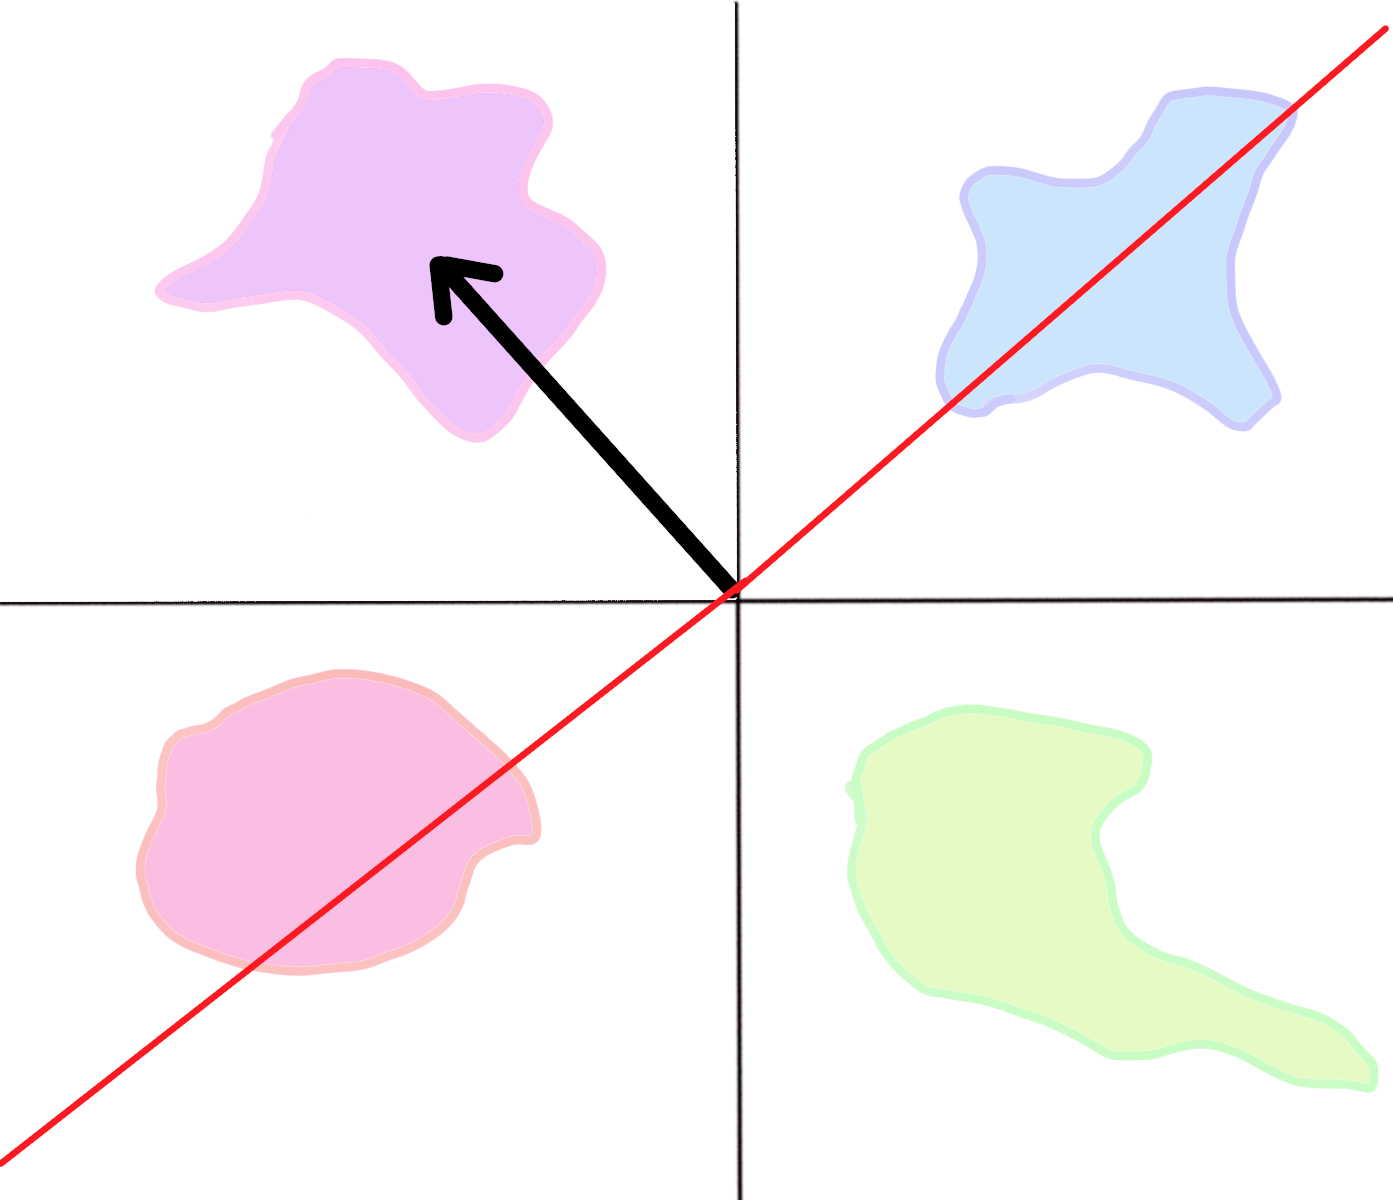
\includegraphics[width=0.8\linewidth]{figures/filter.png}
  \end{center}
  \caption{Filter learned from clustering.}
  \label{fig:filter}
\end{figure}
\end{comment}


\begin{figure}[!t]
  \centering
  \subfloat[Groups of three classes centered on the origin.]{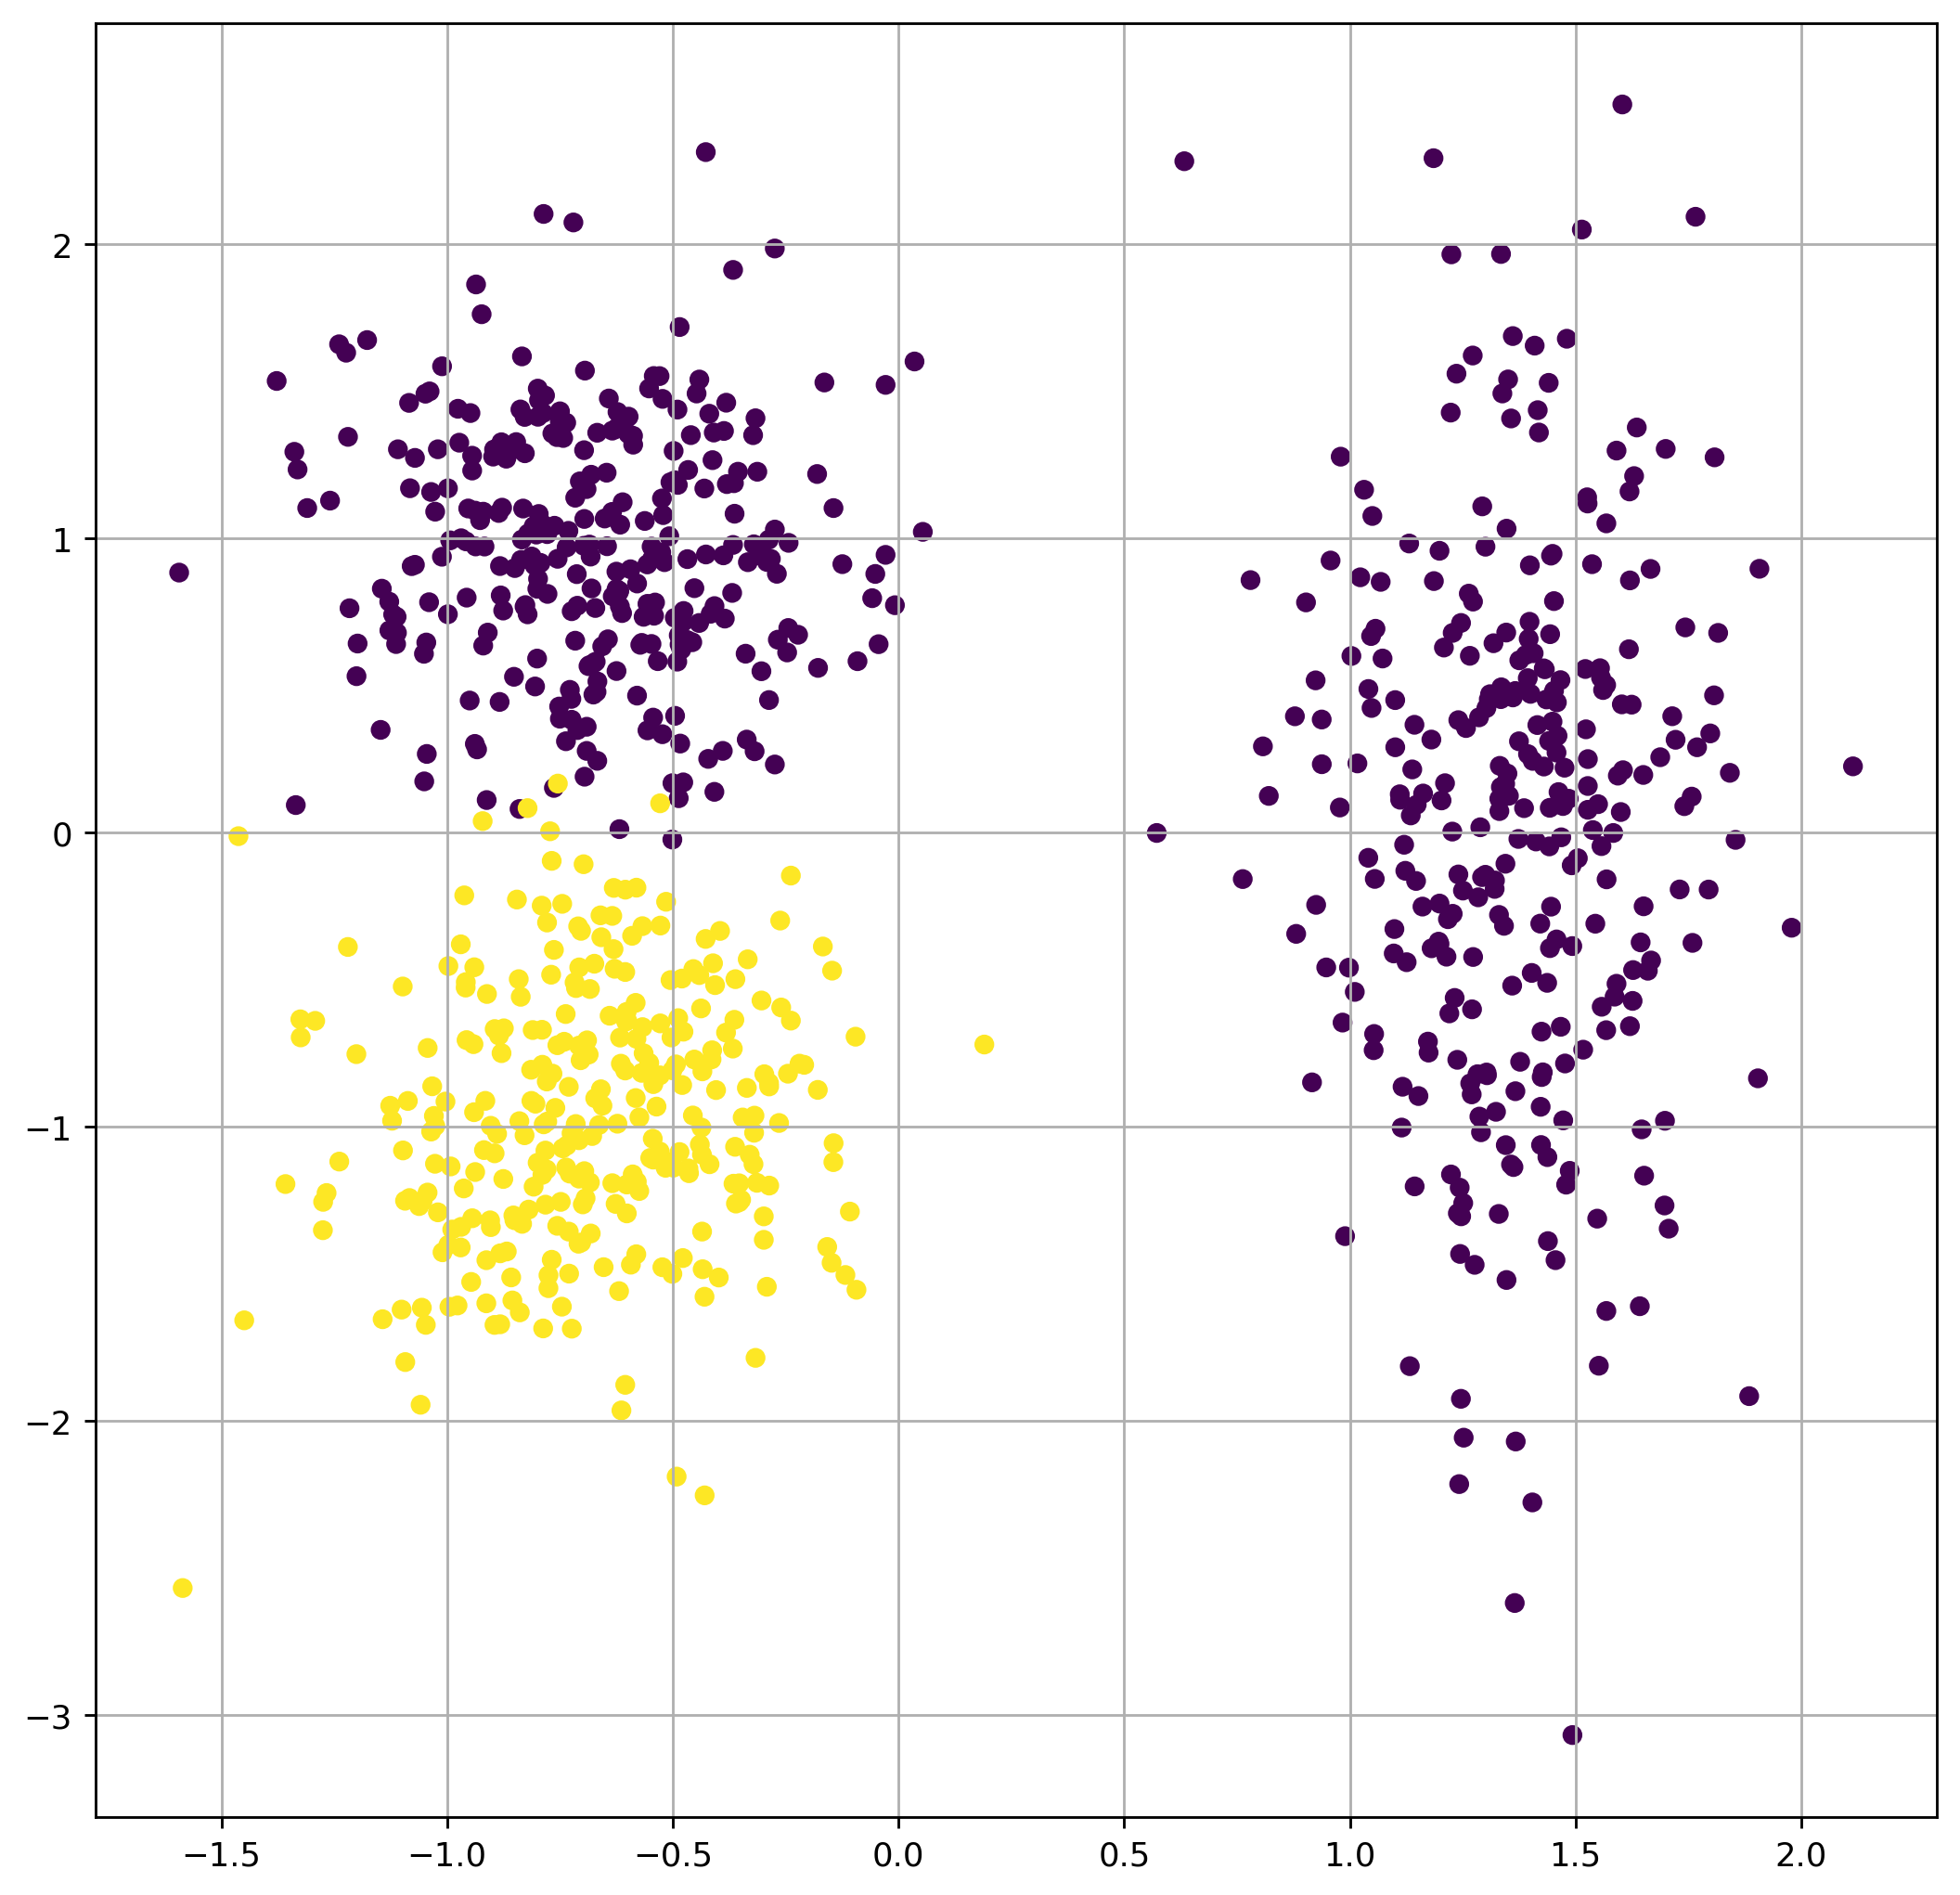
\includegraphics[width=.7\linewidth]{figures/example_groups/groups_centered}}
  \\
  \subfloat[Groups after applying convolution and activation operations.]{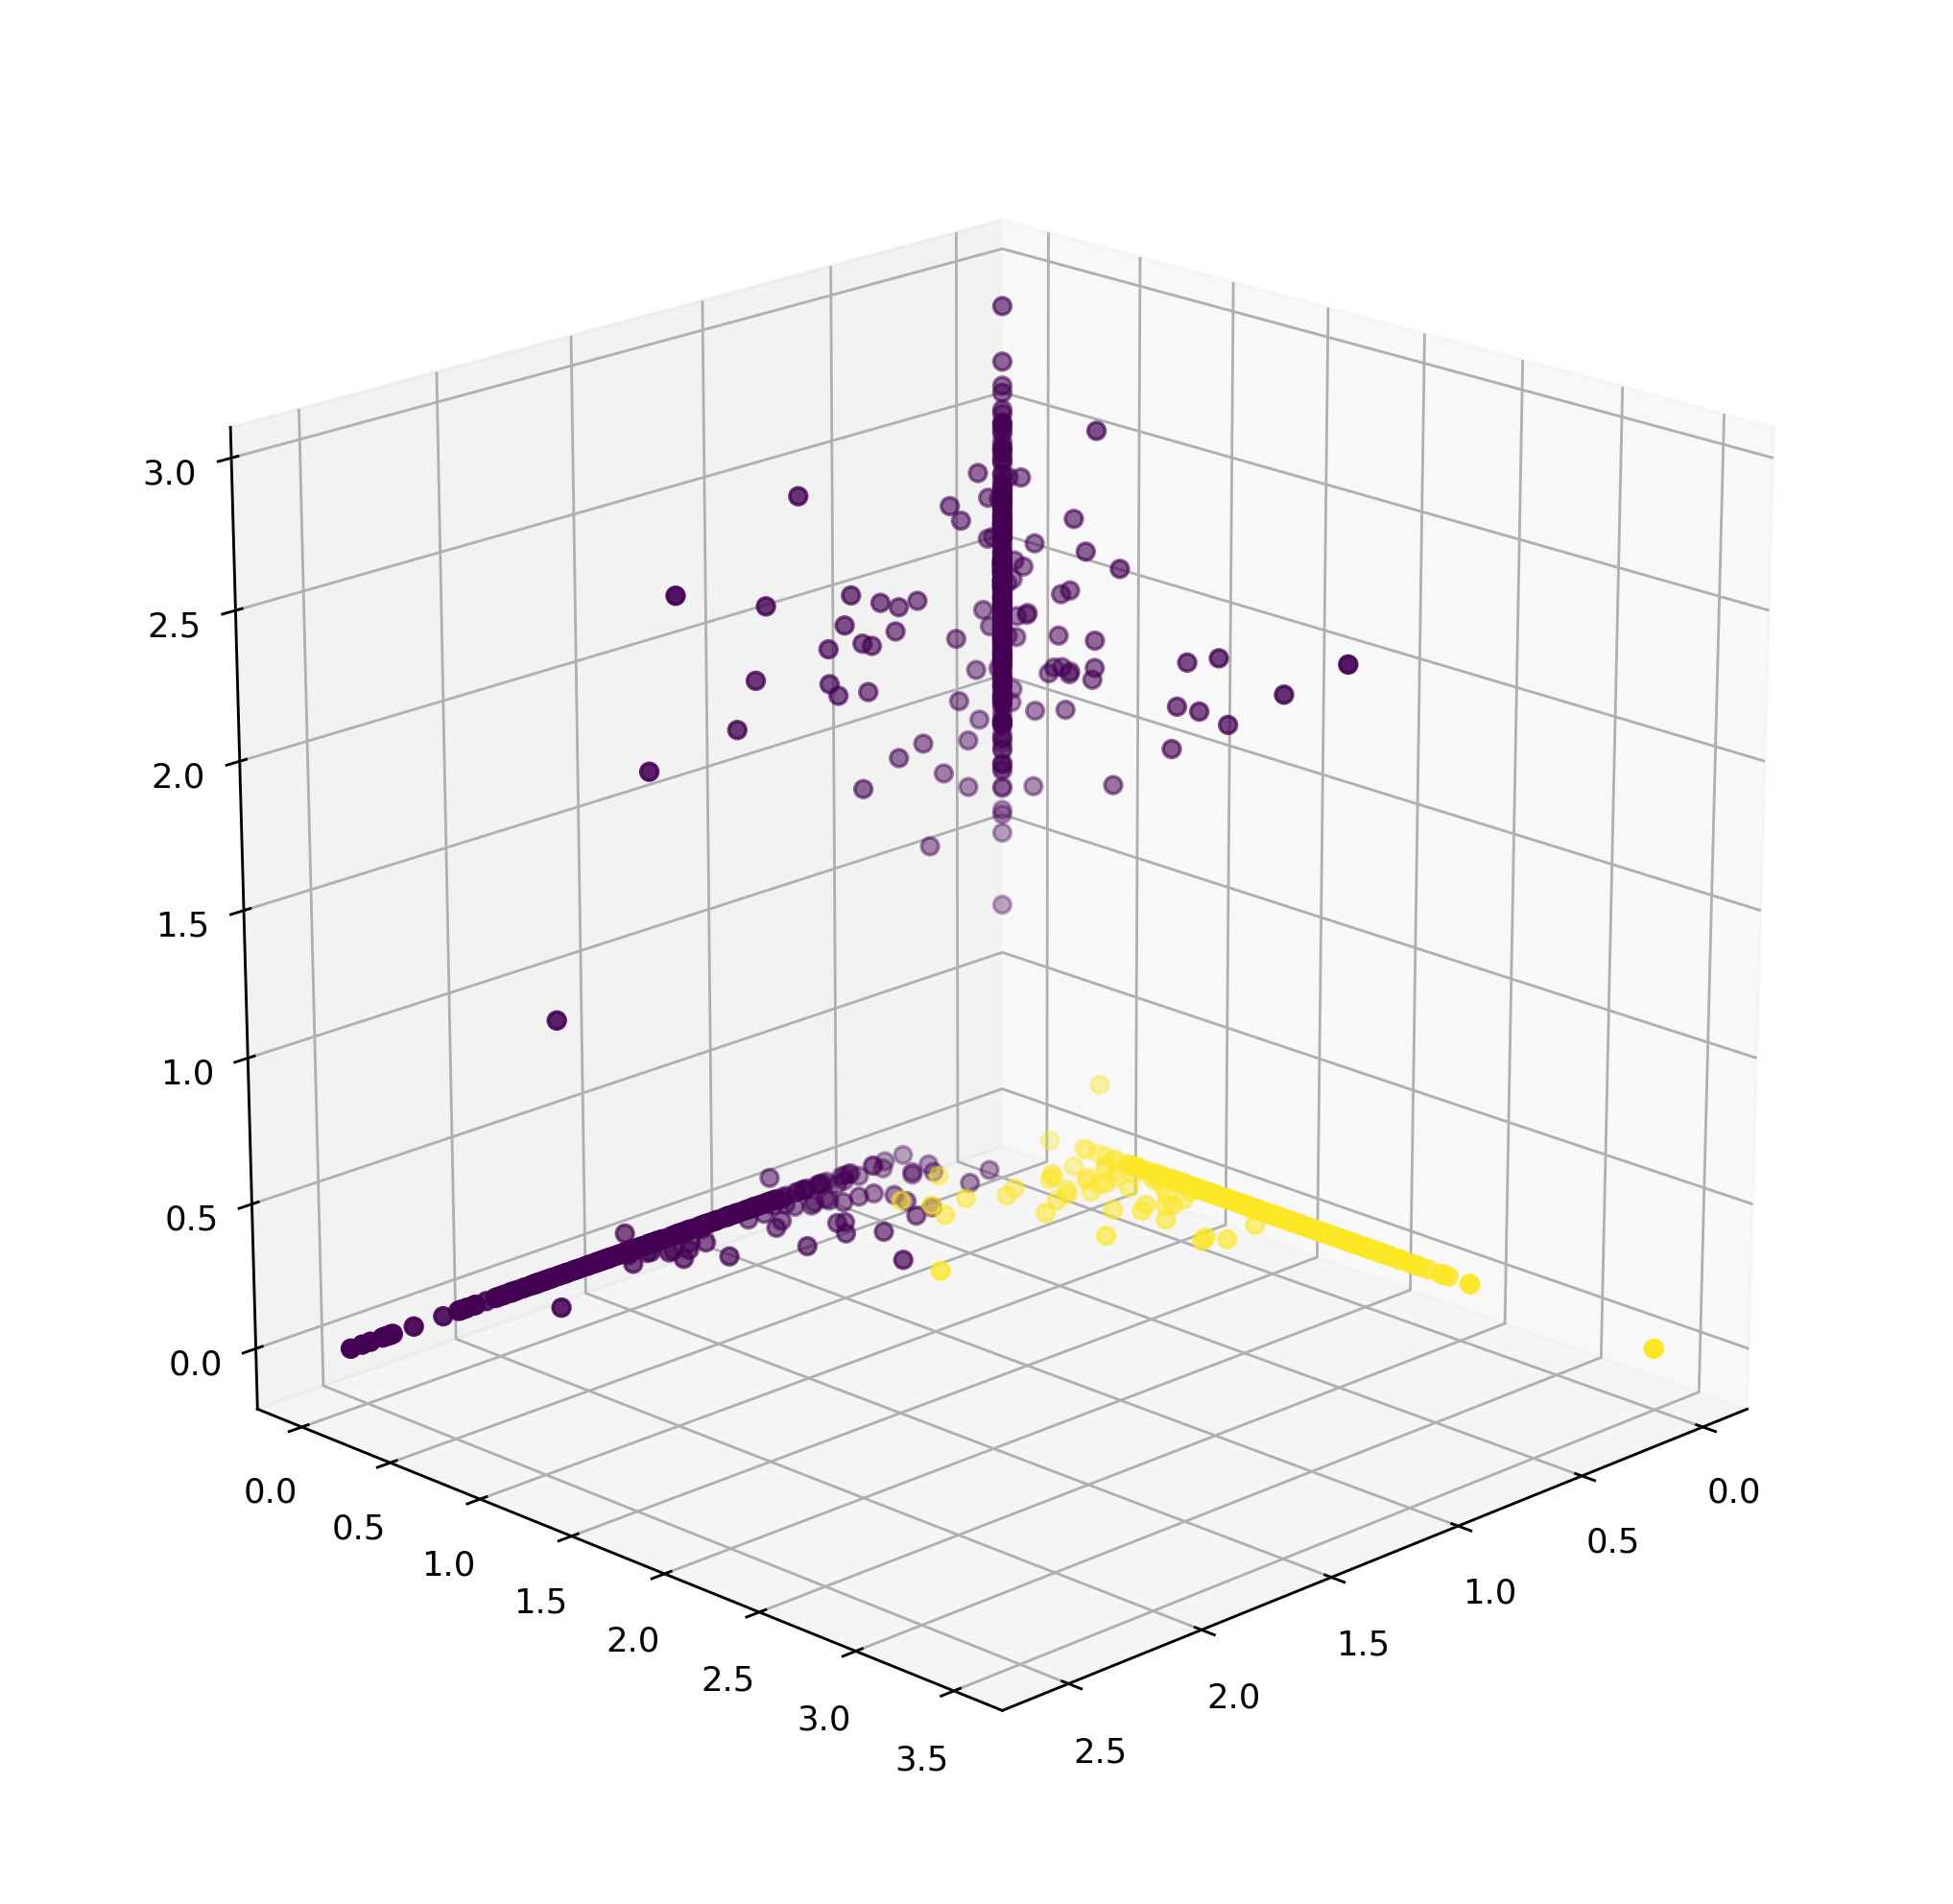
\includegraphics[width=.7\linewidth]{figures/example_groups/groups3d_centered}
  \label{fig_second_case}}
  \caption{Exemple of application of convolution with groups centers as filters' weightes.}
  \label{fig:filter}
\end{figure}


Note that the convolution in a spel $p \in D$ corresponds to the doct product of the locally extended feature vecture and the vector that represents the filter. Thus, let $H$ be a hyperplane orthogonal to the vector of a $\mF$ filter. Thus, let $ H $ be a hyperplane orthogonal to the vector of a $ \mF$ filter. Vectors similar to the vector of filter $\mF$ must fall on the same side of the hyperplane as $\mF$. That is, if the vector $\E(p)$ is on the same side of $H$ as $\mF$, then the doct product between $\E (p)$ and $\mF$ is positive, and is negative otherwise. Thus, the doct product between the center of a cluster and each of the vectors of that cluster must be positive, which implies that the center is a good filter to identify the pattern described by that cluster. In the Figure \ref{fig:filter} we can see an example.

Since all the patches used to produce the filters are centered around the origin, as well as the images of $\D$, we have that the hyperplanes ortogonal to the filters contain the origin, therefor there is no need for bias.

Each convolutional layer is trained individually, one layer at a time. After the convolution operation, we apply the ReLU function to eliminate negative activations and the max pooling operation to aggregate local information. We preserve the output dimensions of convolutional layers so that we can use the same markers used in the previous layer. The new patches are generated from the convolutional layer output and the whole process is repeated to find the filters of the next layer.

To exemplify how our method works, we apply it to the problem of segmenting rock images into vegetation, rock and fractures. In Figure we can see an example of the markers added by the network designer in regions that she considers relevant to characterize each of the classes.

\section{Experiments}
To evaluate our method in a quantitative way, we need a dataset with a ground truth and unfortunately the rock image dataset was not properly labeled.

So, we chose to use a dataset formed from patches of coconut images. The dataset consists of images of dimensions $90 \times 90$ of coconut and non-coconut. The latter class having a large variability. The problem of interest is to classify the images in one of the two classes.

As in reality, labeling images is a costly and time-consuming process, we assume that we only knew the true labels of a small set of samples (one hundred images for each class, totaling two hundred images). That way, we would have only those two hundred images to train any models that we would use to try to solve the problem.

To reduce the impact of chance on the results, we randomly selected three sets of 200 images for training and three sets of 11387 images for testing. We wanted to represent a scenario where the network designer did not have much effort to annotate all these images.

From each of these sets of training images, we selected 4 images using the 2D space projection of the 200 images using the tSNE. We tried to select images that were part of more cohesive groups. Thus, these images are more likely to have characteristics that represent their group.

\begin{figure}[!t]
    \centering
    \subfloat[Markers on an image which contains a coconut tree.]{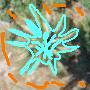
\includegraphics[width=.45\linewidth]{figures/markers1}
    \label{fig:markers1}}
    ~
    \subfloat[Markers on an image which does not contain a coconut tree.]{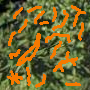
\includegraphics[width=.45\linewidth]{figures/markers2}
    \label{fig:markers2}}
    \\
    \subfloat[Markers on an image which does not contain a coconut tree.]{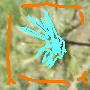
\includegraphics[width=.45\linewidth]{figures/markers3}
    \label{fig:markers3}}
    ~
    \subfloat[Markers on an image which does not contain a coconut tree.]{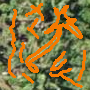
\includegraphics[width=.45\linewidth]{figures/markers4}
    \label{fig:markers4}}
    \caption{Markers used for training.}
\end{figure}

We placed markers on these images in regions that we consider important to identify the coconut and non-coconut (more diverse) classes. An example of a coconut tree image with markers can be seen in Figure \ref{fig:markers1} and non-coconut tree image with markers in Figure \ref{fig:markers2}.

With the markers, we created a convolutional layer with filters of dimensions $7 \times 7$. We did a padding to preserve the dimensions of the images. The network architecture can be seen in the Figure. We used a classifier similar to that of VGG-16.

For clustering to find the convolutional layer filters, we used K-means to cluster the coconut tree patches in 35 clusters and the non-coconut tree patches in also 35 clusters.

\begin{figure}
  \centering
  \subfloat[Visualization of original image feature space.]{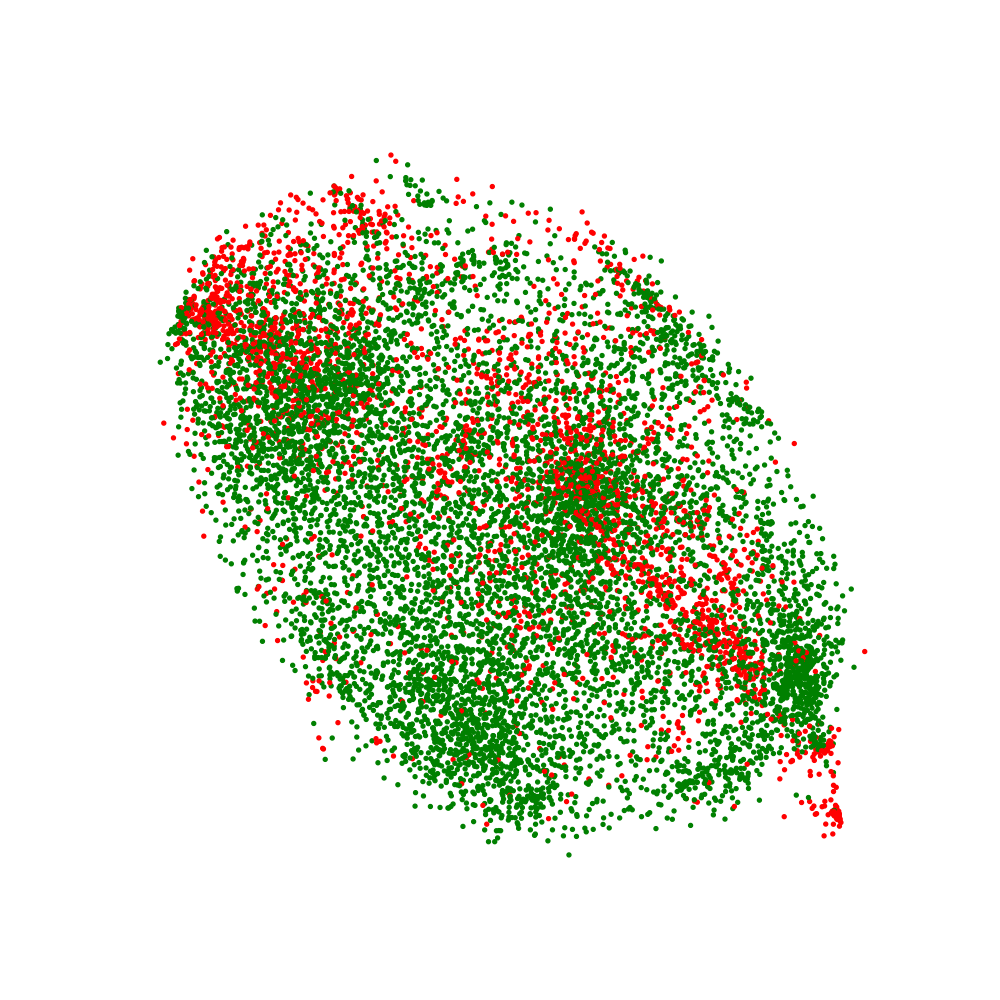
\includegraphics[width=.45\linewidth]{figures/input}
  \label{fig:vis-input}}
  ~
  \subfloat[Visualization of the feature extractor's outputs.]{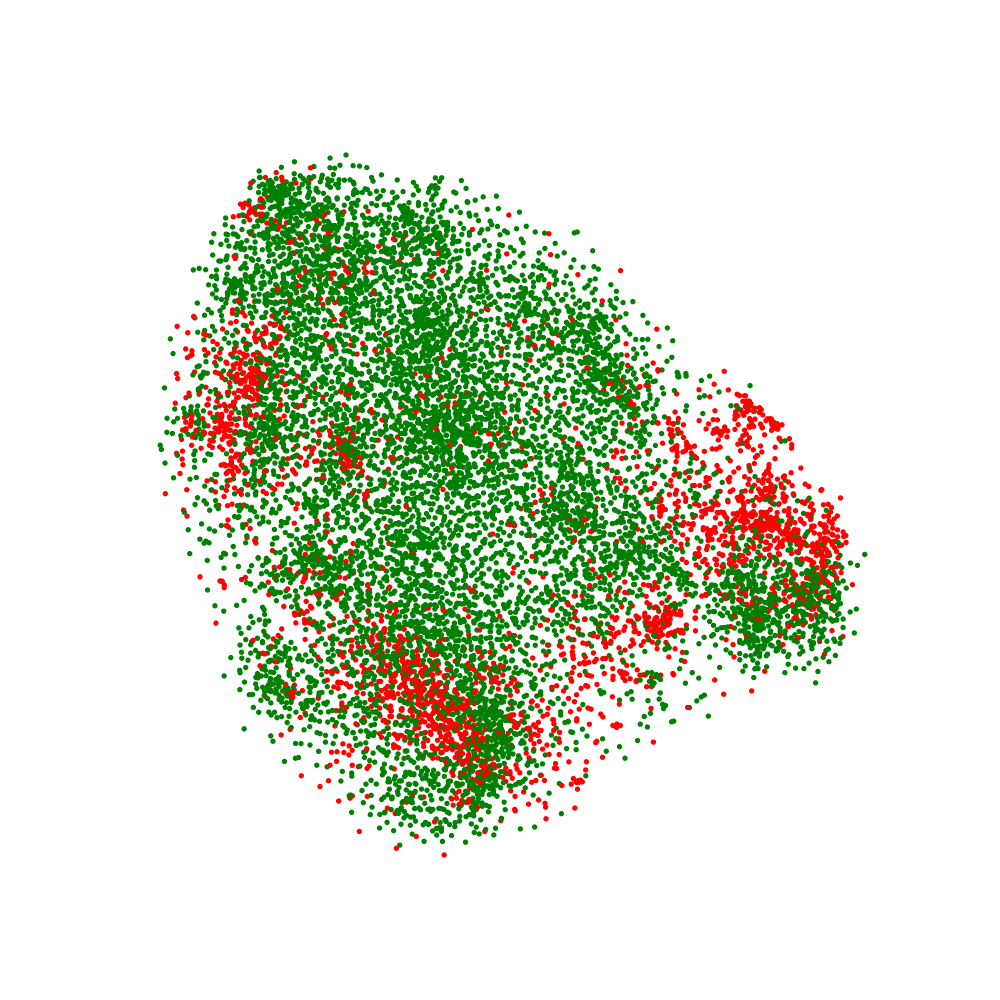
\includegraphics[width=.45\linewidth]{figures/feature_extractor}
  \label{fig:vis-feature-extractor}}
  \\
  \subfloat[Visualization of outputs from the last classifier hidden layer.]{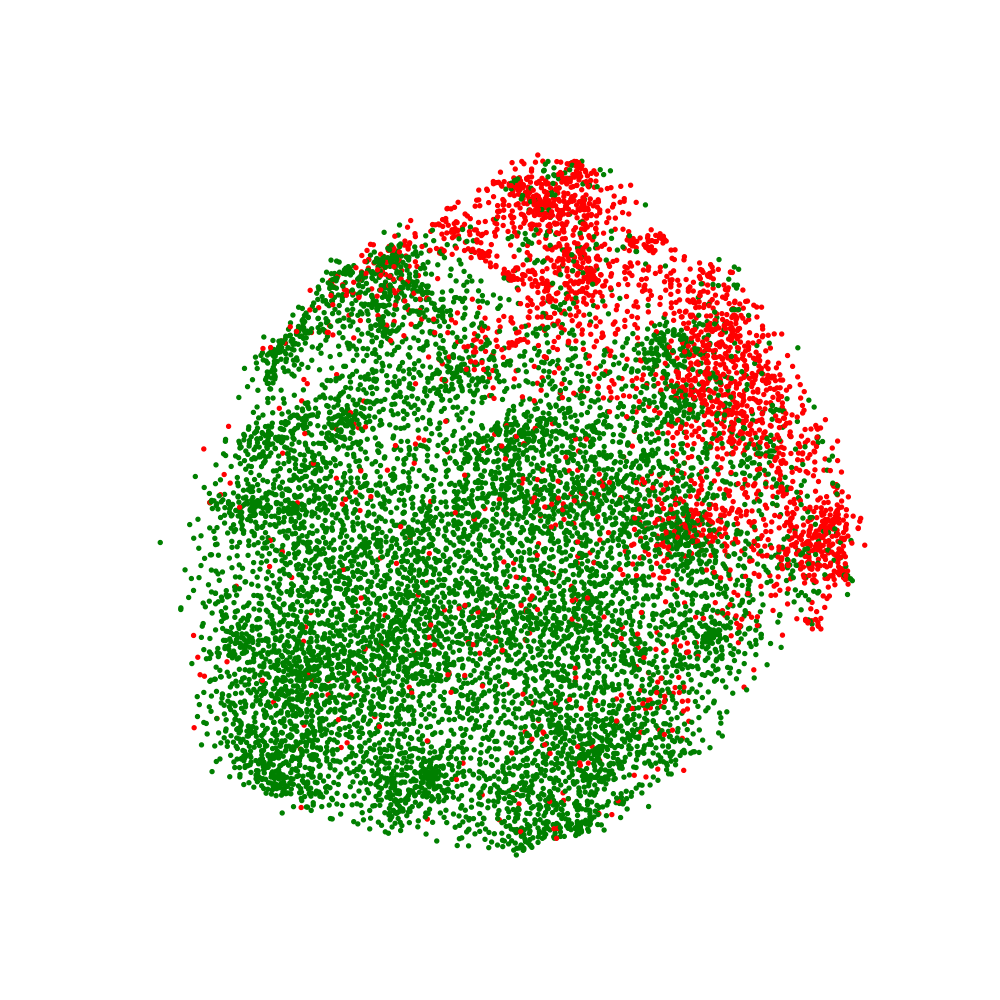
\includegraphics[width=.45\linewidth]{figures/classifier}
  \label{fig:vis-classifier}}
  \caption{This image shows visualizations of the input images and the intermediate layer's outputs. Green points represent background images, and red points represent images that have a coconut tree. The projection from high dimensionality space to 2D was made using t-SNE. The original image shows much overlap between the classes; after applying the feature extractor with only one convolutional layer, we can see that the overlapping decreases considerably. Before the decision layer, the last layer put most of the images from one class on one side and the other on the other side.}
\end{figure}

As the experiments were repeated three times, we reported the mean and standard deviation for each of the metrics in the test set. The results can be seen in the Table \ref{tab:results}.

\begin{table}[!t]
  \begin{center}
  \begin{tabular}{|l|c|c|c|}
  \hline
   Method & Precision & Recall & F-score \\
  \hline\hline
    Ours & $\boldsymbol{0.86 \pm 0.01}$ & $0.84 \pm 0.02$ & $0.85 \pm 0.02$\\
  Ours (fine tuned) & $0.86 \pm 0.01$ & $0.84 \pm 0.02$ & $0.84 \pm 0.02$\\
  Ours with SVM & $0.81 \pm 0.02$ & $0.77 \pm 0.03$ & $0.78 \pm 0.02$\\
  VGG-16 & $0.84 \pm 0.01$ & $0.76 \pm 0.03$ & $0.77 \pm 0.02 $ \\
  VGG-16 (fine tuned) & $0.84 \pm 0.01$ & $0.75 \pm 0.03$ & $0.77 \pm 0.02 $ \\
  \hline
  \end{tabular}
  \end{center}
  \caption{Results.}
  \label{tab:results}
\end{table}

\section{Conclusions}

\bibliographystyle{IEEEtran}
\bibliography{bibliography}

\end{document}


